%! TEX program = xelatex
\documentclass[withoutpreface]{cumcmthesis}

\usepackage{etoolbox}
\usepackage{amsmath,amssymb,mathtools}
\usepackage{booktabs}
\usepackage{tabularx}
\usepackage{array}
\usepackage{multirow}
\usepackage{graphicx}
\usepackage{float}
\usepackage{subcaption}
\usepackage{enumitem}
\usepackage{url}
\usepackage{listings}
\usepackage{xcolor}

\newcolumntype{L}{>{\raggedright\arraybackslash}X}
\newcolumntype{C}{>{\centering\arraybackslash}X}
\newcolumntype{R}{>{\raggedleft\arraybackslash}X}
\graphicspath{{../figures/}}
\setlength{\tabcolsep}{5pt}
\renewcommand{\arraystretch}{1.15}
\captionsetup{font=small}
\captionsetup[subfigure]{font=small}

\title{基于信息时序与滚动优化的微网购电—储能协同调控策略}
\tihao{C}
\baominghao{}
\schoolname{}
\membera{}
\memberb{}
\memberc{}
\supervisor{}
\yearinput{2026}
\monthinput{09}
\dayinput{}

\begin{document}
\maketitle

\begin{abstract}
微网调度同时受到负载、光伏出力、储能状态和电价的共同影响；若把事后实际光伏直接当作日初已知量，虽然容易得到较低的计算费用，却会掩盖计划偏差和紧急购电的真实代价。本文以题目给出的信息发布时间为边界，建立“预测—计划—调整—实时补偿”一致的微网调控模型，在满足负载供电、储能容量、充放电功率和效率约束的前提下，最小化购电结算费用与紧急购电费用。

针对问题一，使用附件1的代表日价格、负载和光伏预测，建立带周期储能边界的线性规划模型。计算得到全天计划购电量为 $59482.6990\ \mathrm{kWh}$、购电费为 $35126.9486\ \mathrm{元}$；储能量始终位于 $[1200,10800]\ \mathrm{kWh}$，并在 0:00 与 24:00 均为 $6000\ \mathrm{kWh}$。

针对问题二，考虑到题面没有提供逐日光伏预报，采用附件1代表日光伏曲线作为日初预测，实际负载曲线作为已知日程，附件2实际光伏仅用于运行阶段。计划购电量日内锁定，储能根据实际光伏做实时修正，短缺部分按 5 倍电价紧急购电。2025年2月1日至12月31日累计紧急购电量为 $1.2255\times10^6\ \mathrm{kWh}$。

针对问题三，在问题二基础上引入 0:00、6:00、12:00、18:00 的滚动光伏预报。将整点预报用“当前实测值锚定的线性插值”映射到十分钟控制网格，并以原计划与调整计划的分段结算费用为目标。使用后续三次预报后，累计紧急购电量由不调整时的 $3.8508\times10^5\ \mathrm{kWh}$ 降至 $1.9293\times10^5\ \mathrm{kWh}$，下降约 $49.9\%$。

针对问题四，将固定日内电价替换为附件4的波动电价，重新执行问题二、问题三的因果调度。波动电价下，问题二和问题三总费用分别为 $1.7961\times10^7$ 元和 $1.3905\times10^7$ 元；滚动预报仍能保持相对稳定的紧急购电水平。本文的主要特点是显式区分信息集与事后实际值、对预测时间尺度转换进行独立验证，并将计划偏差结算与储能实时补偿放入同一条可复现的控制链中。

\keywords{微网调度\quad 储能优化\quad 光伏预测\quad 滚动调整\quad 线性规划}
\end{abstract}
\newpage

\section{问题重述}
\subsection{问题背景}
微网通过光伏等分布式能源和储能设备，在负载侧实现部分能源自给，并通过外部电网补足供电缺口。微网运行的难点不只是“在低价时充电、高价时放电”：光伏具有明显的日内波动，负载和电价随时间变化，储能受容量、功率和效率约束；同时，日初购电计划与运行过程中更新的光伏预报之间存在结算偏差。若日初计划过少，可能触发高价紧急购电；若计划过多，又会产生违约或调整费用。

题目给出 2025 年的十分钟负载、光伏实际出力和电价数据，以及四个时刻发布的逐小时光伏预报。要求以储能初始电量和设备参数为边界，给出购电、充电和放电的可执行策略，并按照结果模板保存完整结果。

\subsection{需要解决的问题}
\begin{enumerate}[itemindent=2em]
    \item 对附件1给出的代表日价格、负载和光伏预测，建立 0:00 制定的全天购电计划，要求供电不低于负载、储能 0:00 与 24:00 电量相同，并给出指定十分钟时段及四小时段统计结果。
    \item 在日内电价曲线每天相同、负载和光伏实际出力随日期变化的情况下，建立日初计划模型；当计划和储能无法满足实际负载时，按交易时刻电价的 5 倍进行紧急购电，并给出 2025 年 2 月 1 日至 12 月 31 日的结果。
    \item 利用 0:00、6:00、12:00、18:00 获得的未来 24 小时整点光伏预报，建立可以滚动调整购电量的模型，处理计划量与调整量之间的 0.5 倍、1.5 倍结算，并判断后续预报是否值得使用。
    \item 将外网电价替换为附件4的十分钟波动电价，重新计算问题二和问题三，并分别保存结果文件。
\end{enumerate}

\section{问题分析}
\subsection{最先需要确定的是信息边界}
本题最容易出现的错误是把附件2中的“实际光伏功率”直接代入 0:00 的计划模型。这样做相当于提前知道全天真实出力，问题二中的紧急购电将失去实际含义，也无法体现问题三的滚动预报价值。因此，本文先把数据按信息发布时间分成三层：日初可用的计划信息、运行时可用的当前状态信息和事后用于评价的实际出力信息。

问题一给出了一条完整的代表日预测曲线，可以直接作为确定性计划输入。问题二没有提供逐日光伏预报，本文将附件1中的代表日光伏曲线作为统一日初预测；当天负载曲线作为已知日程。问题三补充了逐日、逐时刻的光伏预报，因此日初计划使用 0:00 预测，后续时刻只更新尚未发生的控制区间。问题四不改变信息结构，只替换价格过程。

\subsection{四问的递进关系}
问题一先解决一个没有预测误差的基准日内储能套利问题，确定功率平衡、效率和边界的统一写法。问题二把代表日光伏替换为实际日期的运行场景，计划购电量在日初锁定，储能承担第一层误差吸收，剩余缺口才进入紧急购电。问题三增加滚动预报，把原计划与新计划的偏差结算纳入目标，在不回溯修改已经发生时段的条件下重新调度。问题四则检验上述控制逻辑对波动价格的适应性。

\begin{figure}[H]
    \centering
    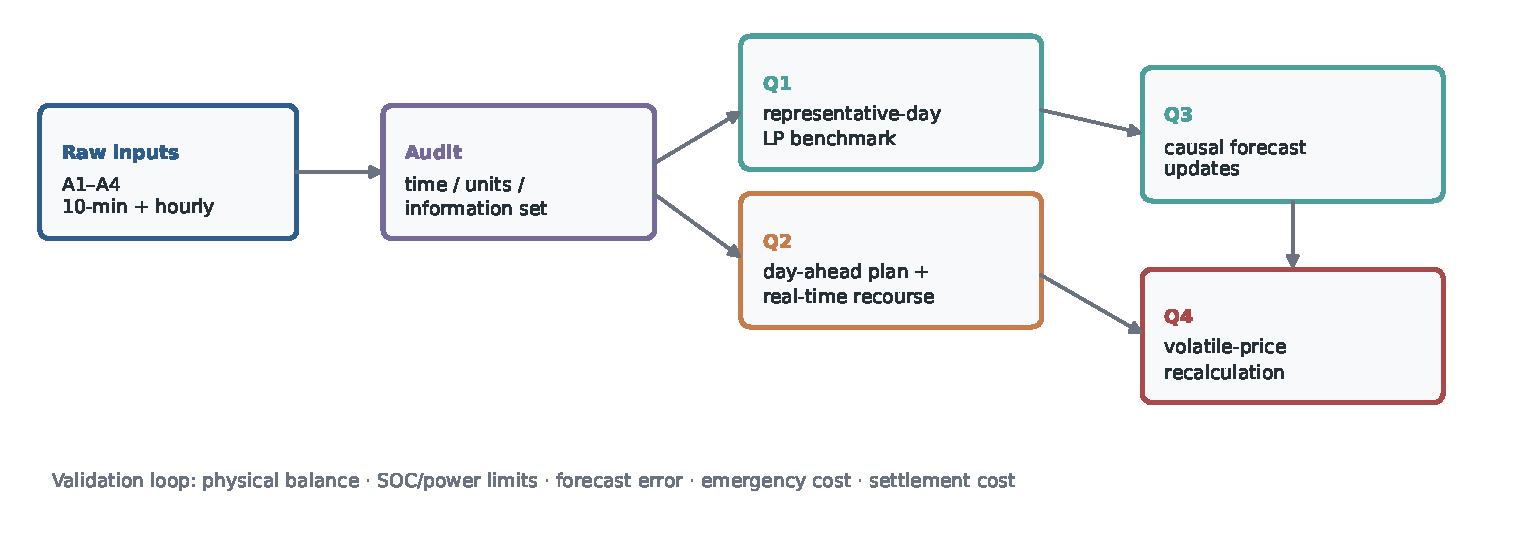
\includegraphics[width=0.98\textwidth]{overview_model.pdf}
    \caption{从信息审计到滚动调度的模型主线}
    \label{fig:overview}
\end{figure}

\subsection{建模选择}
四问的核心变量均为十分钟内的功率或能量，约束为线性平衡、线性储能动态和上下界，因此优先采用线性规划而不是元启发式算法；这种连续优化建模方式也便于对可行域和边界解作透明核验~\cite{boyd2004,rao2016}。问题二和问题三的“智能性”不体现在换用复杂算法，而体现在信息集的正确切分、实际运行阶段的可行补偿以及滚动决策的因果性。对问题三的逐小时预报，先做独立的时间尺度转换误差审计，再把通过验证的转换方式放入优化模型。

\section{模型假设}
\begin{enumerate}[itemindent=2em]
    \item 附件中标为 $00{:}10,\ldots,23{:}50,0{:}00+1$ 的功率和价格分别代表对应十分钟区间的结束时刻；每个区间长度为 $\Delta=1/6\ \mathrm{h}$。
    \item 微网不向外网售电，光伏和购电的剩余部分可以弃光；由于题目没有给出外送价格，弃光不产生收益。
    \item 充电量和放电量按交流侧计量，充放电效率均为 $\eta=0.9$；电池能量必须位于 $[1200,10800]\ \mathrm{kWh}$，充放电功率不超过 $5000\ \mathrm{kW}$。
    \item 日内计划采用周期边界，即当天结束储能量等于当天开始储能量。该假设避免有限时域末端把储能无偿放空，问题一的题面也明确要求此边界；问题二至问题四将其作为日常循环运行的建模假设，并在模型评价中讨论。
    \item 题目没有给出负载预报，本文将当天负载曲线视为 0:00 已知的负载计划；光伏的可用信息严格按各问提供的预测数据处理。
    \item 当计划购电量固定后，储能可以根据已观测的实际光伏在实时阶段调整充放电；如果在物理约束下仍无法供足负载，则由紧急购电变量补足。
    \item 同一时段同时充电和放电在正价格、$\eta<1$ 的条件下被支配，因此连续线性规划解若出现数值层面的同时动作，则以数值容差检查并排除。
\end{enumerate}

\section{符号说明}
\begin{table}[H]
\centering
\caption{主要符号说明}\label{tab:symbols}
\begin{tabularx}{0.95\textwidth}{cLcc}
\toprule
符号 & 含义 & 单位 & 备注\\
\midrule
$k$ & 十分钟区间索引 & -- & $k=1,\ldots,144$\\
$\Delta$ & 单个区间长度 & h & $1/6$\\
$l_k,g_k,p_k$ & 负载、光伏功率和交易电价 & kW, kW, 元/kWh & 输入量\\
$q_k$ & 普通计划/调整购电功率 & kW & 决策量\\
$c_k,d_k$ & 交流侧充电、放电功率 & kW & 决策量\\
$u_k$ & 紧急购电功率 & kW & 运行阶段变量\\
$r_k$ & 弃光或剩余电力功率 & kW & 非负松弛量\\
$e_k$ & 区间边界储能量 & kWh & $1200\le e_k\le10800$\\
$\eta$ & 充放电效率 & -- & $0.9$\\
$q_k^P,q_k^A$ & 原计划和滚动调整购电功率 & kW & 问题三\\
\bottomrule
\end{tabularx}
\end{table}

\section{模型的建立与求解}
\subsection{问题一：代表日确定性购电模型}
\subsubsection{数据特征与时间口径}
附件1包含 144 个十分钟记录，功率单位为 kW，价格单位为元/kWh。附件1的负载和价格曲线与附件2、附件4的全年按时刻均值几乎一致，说明它是一个代表日场景；但附件1在若干清晨和傍晚的小光伏值被置零，因此本文严格使用题目原始值，不自行重算均值。

由功率到能量的换算为 $x_k^{E}=x_k\Delta$。图~\ref{fig:q1profile} 给出代表日三条输入曲线：光伏在白天提供主要的局部供能，价格在早晚和夜间存在明显时段差异，储能因此既有“吸收光伏”的作用，也有“跨时段搬移购电”的作用。

\begin{figure}[H]
    \centering
    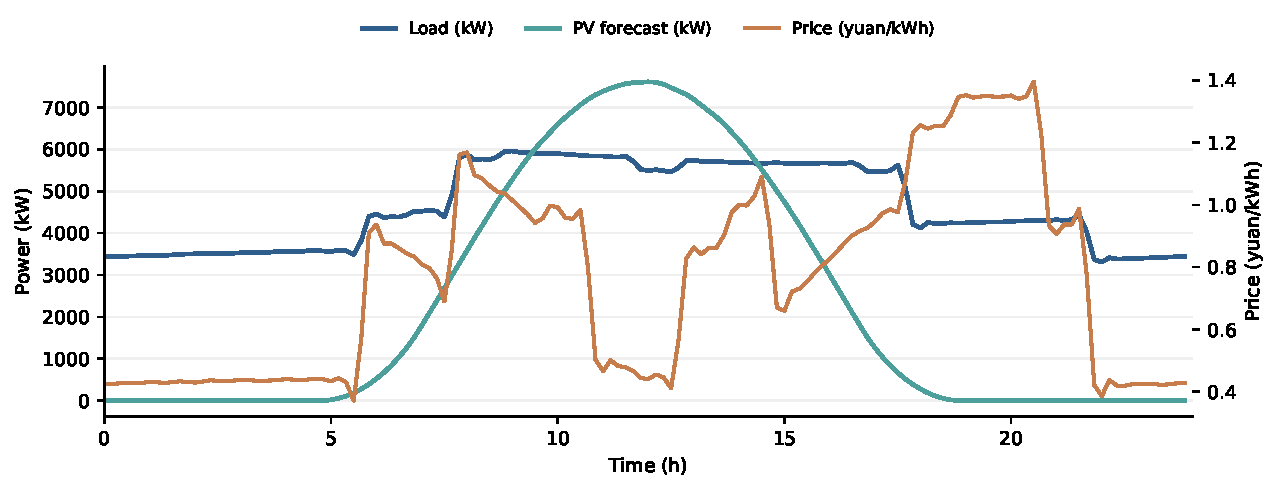
\includegraphics[width=0.86\textwidth]{q1_representative_profile.pdf}
    \caption{附件1代表日负载、光伏预测和电价}
    \label{fig:q1profile}
\end{figure}

\subsubsection{功率平衡和储能动态}
令 $q_k,c_k,d_k,r_k$ 分别为普通购电、充电、放电和弃光功率。问题一没有紧急购电，因此每个十分钟区间满足
\begin{equation}
q_k+g_k+d_k=l_k+c_k+r_k,\qquad k=1,\ldots,144.
\label{eq:q1balance}
\end{equation}

采用交流侧计量，电池能量递推为
\begin{equation}
e_k=e_{k-1}+\eta c_k\Delta-\frac{d_k\Delta}{\eta}.
\label{eq:soc}
\end{equation}

初始和末端电量均为 $6000\ \mathrm{kWh}$。将所有边界条件合并，问题一的优化模型为
\begin{equation}
\boxed{
\begin{aligned}
\min_{q,c,d,r,e}\quad & C_1=\sum_{k=1}^{144}p_kq_k\Delta,\\
\text{s.t.}\quad &q_k+g_k+d_k=l_k+c_k+r_k,\\
&e_k=e_{k-1}+\eta c_k\Delta-d_k\Delta/\eta,\\
&1200\le e_k\le10800,\quad 0\le c_k,d_k\le5000,\\
&q_k,r_k\ge0,\quad e_0=e_{144}=6000.
\end{aligned}}
\label{eq:q1model}
\end{equation}

由于所有购电价格为正且效率小于 1，同时充放电不会降低目标值；求解时不需要额外引入二进制变量。模型是标准线性规划，使用 HiGHS 求解器求解，并在求解后逐时检查式~\eqref{eq:q1balance} 和式~\eqref{eq:soc}。

\subsubsection{问题一结果}
代表日负载和光伏的全天能量分别为 $111024.8081\ \mathrm{kWh}$ 和 $55482.8357\ \mathrm{kWh}$。最优方案的统计量见表~\ref{tab:q1summary}。

\begin{table}[H]
\centering
\caption{问题一全天结果与储能边界检查}\label{tab:q1summary}
\begin{tabular}{l r l r}
\toprule
指标 & 数值 & 指标 & 数值\\
\midrule
全天购电量/kWh & 59482.6990 & 全天购电费/元 & 35126.9486\\
总充电量/kWh & 20740.6661 & 总放电量/kWh & 16799.9396\\
最小储能量/kWh & 1200.0000 & 最大储能量/kWh & 10800.0000\\
0:00储能量/kWh & 6000.0000 & 24:00储能量/kWh & 6000.0000\\
最大充电功率/kW & 5000.0000 & 最大放电功率/kW & 4293.9182\\
弃光量/kWh & 0.0000 & 同时充放电区间 & 0\\
\bottomrule
\end{tabular}
\end{table}

指定时段的购电量和储能动作见表~\ref{tab:q1selected} 和表~\ref{tab:q1storage}。完整 144 个十分钟结果已写入支撑材料中的 \texttt{results/result1.xlsx}；输出文件将模板中错后一格的时间标签改为与 0:00/24:00 边界一致的 \texttt{0:00-0:10} 至 \texttt{23:50-24:00}，避免把数据向未来无声平移。

\begin{table}[H]
\centering
\caption{问题一指定十分钟时段购电量}\label{tab:q1selected}
\begin{tabular}{lrrrrrr}
\toprule
时间段 & 10:00--10:10 & 12:00--12:10 & 14:00--14:10 & 16:00--16:10 & 18:00--18:10 & 20:00--20:10\\
\midrule
购电量/kWh & 0.0000 & 480.4124 & 0.0000 & 445.4317 & 531.8940 & 0.0000\\
\bottomrule
\end{tabular}
\end{table}

\begin{table}[H]
\centering
\caption{问题一四小时段充放电量}\label{tab:q1storage}
\begin{tabular}{lrr}
\toprule
时间段 & 充电量/kWh & 放电量/kWh\\
\midrule
00:00--04:00 & 4500.0000 & 0.0000\\
04:00--08:00 & 833.3333 & 6365.8412\\
08:00--12:00 & 4787.9643 & 1702.9970\\
12:00--16:00 & 5286.0352 & 91.1014\\
16:00--20:00 & 0.0000 & 5780.1319\\
20:00--24:00 & 5333.3333 & 2859.8681\\
\midrule
0:00/24:00储能量 & 6000.0000 & 6000.0000\\
\bottomrule
\end{tabular}
\end{table}

\begin{figure}[H]
    \centering
    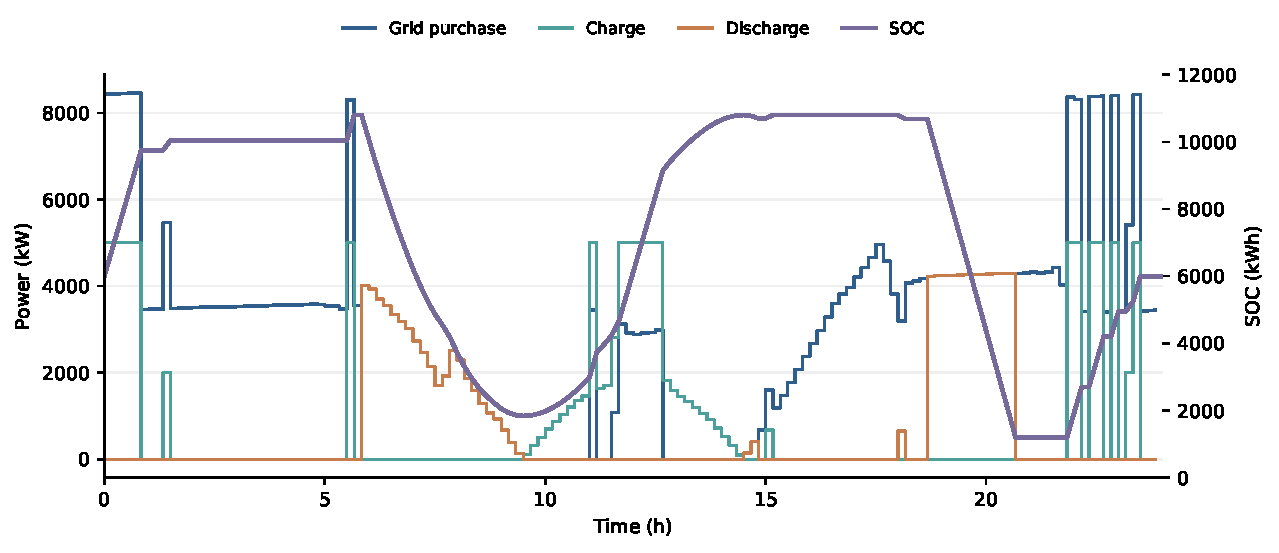
\includegraphics[width=0.86\textwidth]{q1_optimal_dispatch.pdf}
    \caption{问题一最优购电—储能联合调度}
    \label{fig:q1dispatch}
\end{figure}

图~\ref{fig:q1dispatch} 中，储能量在低价或光伏较强时上升，在高价和光伏不足时下降，并在 24:00 回到初值。最优解触及 1200 和 10800 kWh 两个边界，说明储能容量而非单纯的价格差是该代表日的有效约束。

\subsection{问题二：日初计划与实际运行补偿}
\subsubsection{信息集与预测输入}
问题二没有给出逐日光伏预测文件。如果直接使用附件2当天实际光伏，等价于把未来信息泄露给 0:00 的决策。本文的主口径为：当天负载曲线作为日初已知的负载日程，附件1光伏预测作为通用日初光伏预测，附件2实际光伏只在运行阶段用于检验计划是否足够。问题二的计划输入为
\[
\hat l_{d,k}=l_{d,k},\qquad \hat g_{d,k}=g^{(1)}_k,
\]
其中 $d$ 为日期，$g^{(1)}$ 为附件1光伏预测曲线。

\subsubsection{日初计划模型}
对每个日期 $d$，用式~\eqref{eq:q1model} 的结构，以 $\hat l_{d,k},\hat g_{d,k}$ 和附件1价格 $p_k$ 求解 $q^P_{d,k}$。计划量一旦在 0:00 生成，日内不再修改。为避免日末效应，令 $e_{d,144}=e_{d,0}$。

运行阶段观测到实际光伏 $g_{d,k}^{\mathrm{act}}$ 后，固定 $q^P_{d,k}$，允许储能重新选择 $c_{d,k},d_{d,k}$。定义 $u_{d,k}$ 为紧急购电功率、$r_{d,k}$ 为弃光功率，则
\begin{equation}
q^P_{d,k}+g^{\mathrm{act}}_{d,k}+d_{d,k}+u_{d,k}
=l_{d,k}+c_{d,k}+r_{d,k}.
\label{eq:q2realbalance}
\end{equation}

实时补偿模型以紧急购电费用为主目标：
\begin{equation}
\boxed{
\begin{aligned}
\min_{c,d,r,u,e}\quad & C_{2,d}=\sum_{k=1}^{144}5p_k u_{d,k}\Delta,\\
\text{s.t.}\quad &\text{式~\eqref{eq:q2realbalance}及式~\eqref{eq:soc}},\\
&1200\le e_{d,k}\le10800,\quad 0\le c_{d,k},d_{d,k}\le5000,\\
&e_{d,0}=e_{d,144}=6000,\quad u_{d,k},r_{d,k}\ge0.
\end{aligned}}
\label{eq:q2model}
\end{equation}

实际储能动作由该实时模型输出，计划购电量仍保持为 $q^P$。2025 年 1 月用同一策略作为状态暖机期，结果文件按题目模板从 2 月 1 日开始列示。

\subsubsection{问题二结果与反误导对照}
2025 年 2 月 1 日至 12 月 31 日共 334 天的累计结果见表~\ref{tab:q2total}。紧急购电量较大的日期集中在实际光伏明显低于代表日预测的时段；例如 12 月 21 日冬季日照不足，紧急购电量显著增加。

\begin{table}[H]
\centering
\caption{问题二与问题三的全年累计结果（固定日内价格）}\label{tab:q2total}
\begin{tabular}{lrrrr}
\toprule
方案 & 计划/结算费用/元 & 调整费用/元 & 紧急费用/元 & 紧急购电量/kWh\\
\midrule
问题二：日初计划 & 12352438.4401 & -- & 4521889.5482 & 1225461.4206\\
问题三：滚动调整 & 12572629.8488 & 224829.6877 & 697379.0133 & 192929.1083\\
\bottomrule
\end{tabular}
\end{table}

如果把当天实际光伏直接作为问题二的日初预测，334 天紧急购电量为 0；如果同时使用代表日负载和代表日光伏，紧急购电量反而上升到约 $3.0652\times10^6\ \mathrm{kWh}$。这两个对照说明，信息集选择比换用更复杂的算法更关键。本文不把完美预知结果作为答案，只把它作为数据泄漏的诊断基线。

\begin{table}[H]
\centering
\caption{问题二指定日期紧急购电结果}\label{tab:q2target}
\begin{tabular}{lrrr}
\toprule
日期 & 计划费用/元 & 紧急购电量/kWh & 紧急费用/元\\
\midrule
2025.3.20 & 39774.8731 & 558.5877 & 2853.6653\\
2025.6.21 & 21004.6721 & 0.0000 & 0.0000\\
2025.9.23 & 43240.1615 & 359.1406 & 2011.6673\\
2025.12.21 & 44003.4435 & 20545.2160 & 78345.5163\\
\bottomrule
\end{tabular}
\end{table}

完整计划、实际储能动作和连续紧急购电区间分别写入 \texttt{results/result2.xlsx}。工作簿中的储能表不再保留模板的省略号，而是补齐 334 天的全部六个四小时段。

\subsection{问题三：因果滚动预报与计划偏差结算}
\subsubsection{逐小时预测到十分钟控制网格}
附件3在每天 0:00、6:00、12:00、18:00 发布未来 24 小时整点预测。设发布时刻为 $r$，预测的第 $h$ 个点为 $\hat g_{r+h}$，其目标时刻为 $r+60h$ 分钟。由于控制变量仍为十分钟功率，本文采用当前发布时刻的实测值作为锚点，并在相邻整点间做线性插值：
\begin{equation}
\hat g(t)=\hat g_{r+h-1}+\frac{t-[r+60(h-1)]}{60}\left(\hat g_{r+h}-\hat g_{r+h-1}\right).
\label{eq:interpolation}
\end{equation}

在 $r=0$ 时，附件没有 0:00 列，锚点取 0；在其他发布时刻，锚点取当前已观测光伏。独立利用全年附件2实际光伏验证后，参考可再生能源预测的运行管理研究~\cite{pinson2013}，线性插值的十分钟 MAE 为 $138.52\ \mathrm{kW}$，零阶保持为 $324.76\ \mathrm{kW}$；因此主模型采用式~\eqref{eq:interpolation}，零阶保持仅作敏感性分析。

\begin{figure}[H]
    \centering
    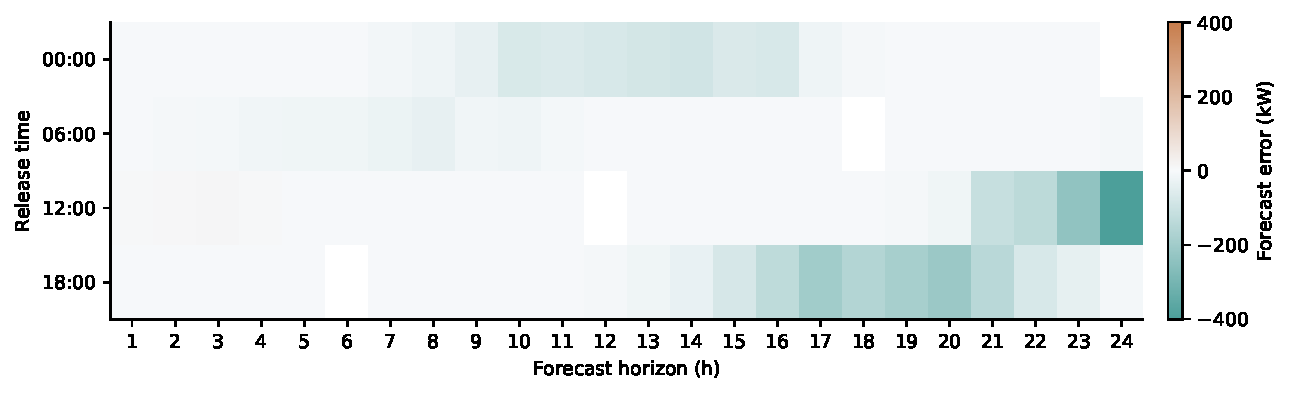
\includegraphics[width=0.91\textwidth]{forecast_error_heatmap.pdf}
    \caption{不同发布时刻与预测时距的平均光伏预测误差}
    \label{fig:forecast_error}
\end{figure}

\subsubsection{调整量与结算费用}
设原计划为 $q^P_k$，根据最新预报得到的调整购电量为 $q^A_k$。把低于计划和高于计划的偏差分别写为
\[
v^-_k=(q^P_k-q^A_k)^+,\qquad v^+_k=(q^A_k-q^P_k)^+.
\]
题目给出的 0.5 倍和 1.5 倍价格可以统一写成连续的分段结算函数
\begin{equation}
\phi_k(q^A_k;q^P_k)=\left[p_kq^A_k+0.5p_k(v^-_k+v^+_k)\right]\Delta.
\label{eq:settlement}
\end{equation}
当 $q^A_k<q^P_k$ 时，式~\eqref{eq:settlement} 等价于实际执行量按原价、未执行部分按 0.5 倍价格结算；当 $q^A_k>q^P_k$ 时，等价于原计划按原价、超出部分按 1.5 倍价格结算。

在发布时刻 $r$，仅对 $r$ 之后尚未发生的区间重新优化，原计划在更早区间保持不变；这种“日初计划—平衡调整”的结构与含随机出力的电力市场调度文献中的分层结算思想相近~\cite{morales2014}。对剩余区间，调整模型为
\begin{equation}
\boxed{
\begin{aligned}
\min_{q^A,c,d,r,u,e,v^-,v^+}\quad
&\sum_{k\ge r}\left[\phi_k(q^A_k;q^P_k)+5p_ku_k\Delta\right],\\
\text{s.t.}\quad
&q^A_k+\hat g_{r,k}+d_k+u_k=l_k+c_k+r_k,\\
&q^A_k=q^P_k-v^-_k+v^+_k,\\
&e_k=e_{k-1}+\eta c_k\Delta-d_k\Delta/\eta,\\
&1200\le e_k\le10800,\quad 0\le c_k,d_k\le5000,\\
&q^A_k,r_k,u_k,v^-_k,v^+_k\ge0,\quad e_{24:00}=e_{0:00}.
\end{aligned}}
\label{eq:q3model}
\end{equation}

这里的 $\hat g_{r,k}$ 是由最新发布时刻 $r$ 的预测经过式~\eqref{eq:interpolation} 得到的十分钟预测。求解过程按 0:00、6:00、12:00、18:00 依次推进，已经发生的区间不再回溯修改；实际运行时再用附件2的实际光伏求解固定购电量下的储能补偿。

\subsubsection{滚动调整价值}
表~\ref{tab:q3value} 比较了只使用 0:00 预报和使用全部四个发布时刻的结果。后续预报使紧急购电量下降约 $49.9\%$，总费用下降约 $2.73\%$。下降幅度没有与紧急电量完全同步，是因为滚动调整同时带来了计划偏差结算费用。

\begin{table}[H]
\centering
\caption{问题三后续预报的价值}\label{tab:q3value}
\begin{tabular}{lrrrr}
\toprule
策略 & 结算费用/元 & 调整费用/元 & 紧急购电量/kWh & 总费用/元\\
\midrule
只用 0:00 预报 & 12347800.1611 & 0.0000 & 385078.4831 & 13642351.1649\\
使用 0:00/6:00/12:00/18:00 & 12572629.8488 & 224829.6877 & 192929.1083 & 13270008.8621\\
\bottomrule
\end{tabular}
\end{table}

\begin{figure}[H]
    \centering
    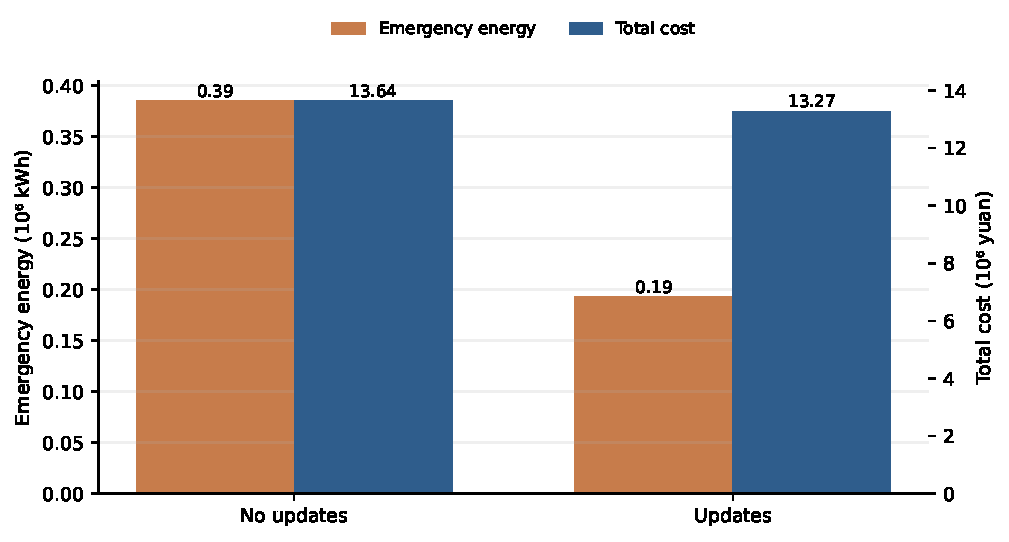
\includegraphics[width=0.72\textwidth]{q3_update_value.pdf}
    \caption{后续预报对紧急购电量和总费用的影响}
    \label{fig:updatevalue}
\end{figure}

\begin{table}[H]
\centering
\caption{问题三指定日期的计划与调整购电量}\label{tab:q3target}
\begin{tabular}{lrrr}
\toprule
日期 & 日初计划购电量/kWh & 最终调整购电量/kWh & 实际紧急购电量/kWh\\
\midrule
2025.3.20 & 67748.6571 & 63896.7334 & 2536.1526\\
2025.6.21 & 33227.8302 & 33385.8392 & 43.4965\\
2025.9.23 & 68433.1745 & 66238.2545 & 241.6891\\
2025.12.21 & 93633.2068 & 93547.9261 & 838.8348\\
\bottomrule
\end{tabular}
\end{table}

以 2025 年 3 月 20 日为例，图~\ref{fig:q3example} 同时画出实际负载、实际光伏、日初计划、最终调整和储能状态。可以看到，调整主要发生在光伏爬升和衰减区间，储能状态仍保持在允许区间内；这说明后续预报的作用是修正功率时序，而不是简单增加全天购电量。

\begin{figure}[H]
    \centering
    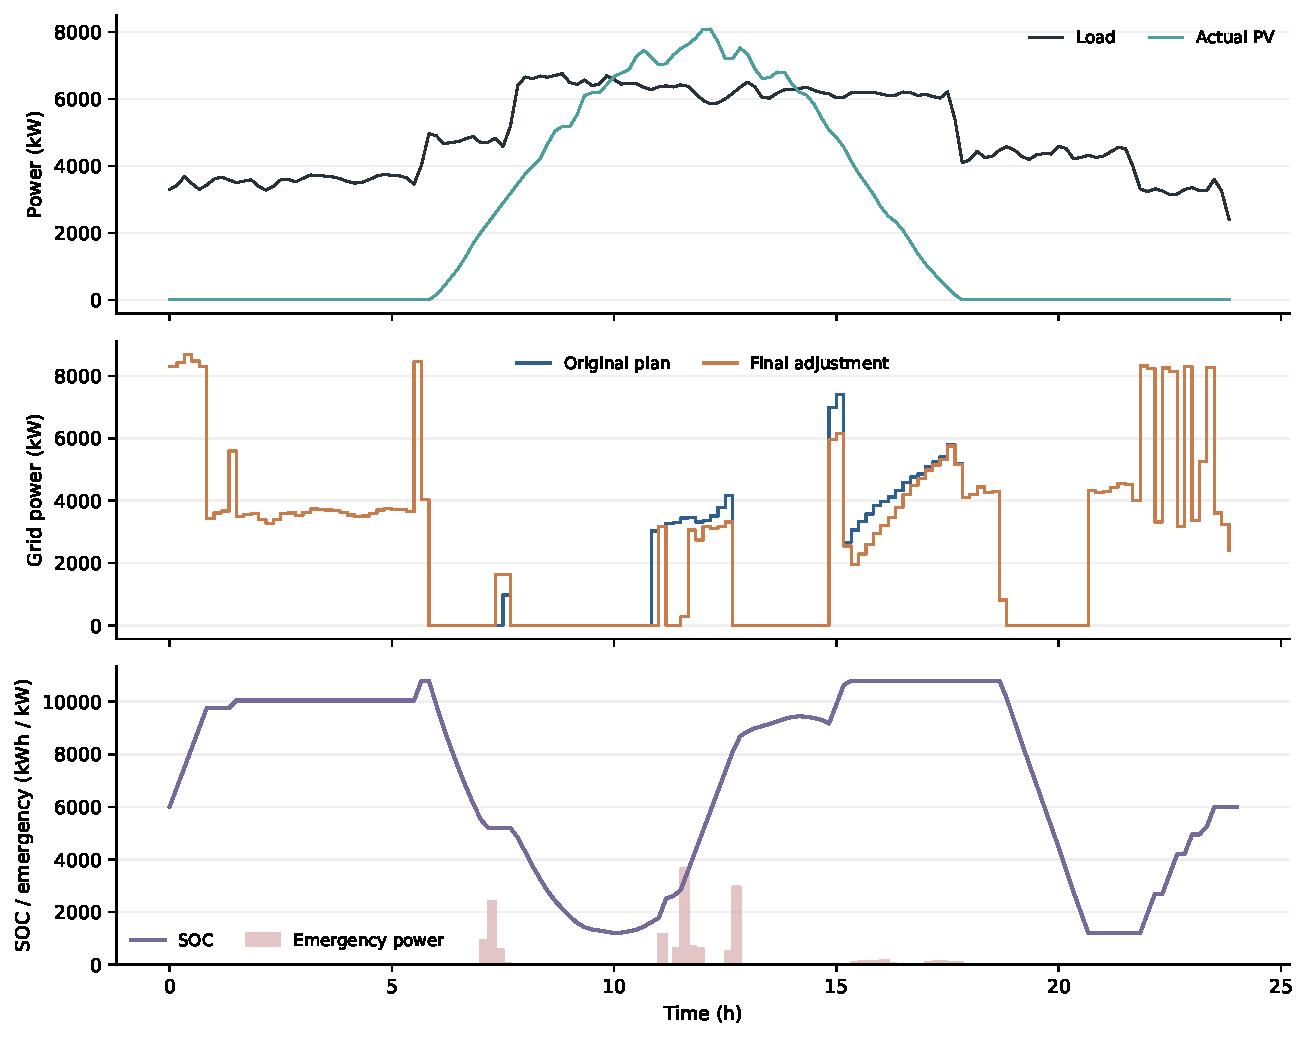
\includegraphics[width=0.86\textwidth]{q3_example_day.pdf}
    \caption{2025 年 3 月 20 日的因果滚动调度示例}
    \label{fig:q3example}
\end{figure}

\subsection{问题四：波动电价下的重新计算}
\subsubsection{价格过程替换}
问题四不改变问题二和问题三的预测信息与控制时序，只将固定日内价格 $p_k$ 替换为附件4中对应日期的波动价格 $p_{d,k}^{\mathrm{vol}}$。因此，问题二的计划费用和紧急费用分别替换为
\[
C_{4-2}=\sum_{d,k}p_{d,k}^{\mathrm{vol}}q^P_{d,k}\Delta+5\sum_{d,k}p_{d,k}^{\mathrm{vol}}u_{d,k}\Delta,
\]
问题三则把式~\eqref{eq:settlement} 中的 $p_k$ 替换为 $p_{d,k}^{\mathrm{vol}}$。

\begin{table}[H]
\centering
\caption{固定价格与波动价格下的全年总费用}\label{tab:q4}
\begin{tabular}{lrrr}
\toprule
方案 & 固定日内价格/元 & 波动价格/元 & 变化比例\\
\midrule
问题二：日初计划 & 16874327.9883 & 17960780.5468 & $+6.44\%$\\
问题三：滚动调整 & 13270008.8621 & 13904585.0292 & $+4.78\%$\\
\bottomrule
\end{tabular}
\end{table}

波动价格下问题二的紧急购电量为 $1.21596\times10^6\ \mathrm{kWh}$，问题三为 $1.94091\times10^5\ \mathrm{kWh}$。问题三的滚动预报仍明显减少紧急购电，说明信息更新的价值并不依赖固定价格这一特殊设定。

\begin{figure}[H]
    \centering
    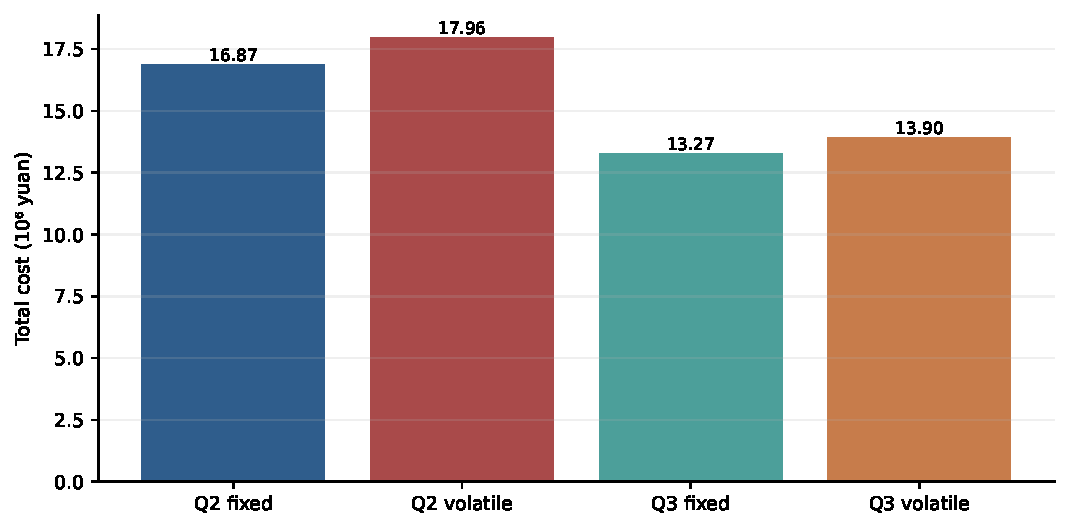
\includegraphics[width=0.72\textwidth]{q4_price_comparison.pdf}
    \caption{两种价格机制下四类方案的总费用}
    \label{fig:q4}
\end{figure}

\section{模型评价与推广}
\subsection{模型优点}
\begin{enumerate}[itemindent=2em]
    \item \textbf{信息边界清晰。}模型不把事后实际光伏倒灌进日初计划，问题二、问题三的紧急购电结果因此具有实际含义。
    \item \textbf{物理约束可核验。}所有结果都由功率平衡、储能递推、容量上下界和充放电功率上限共同产生；代码对每个区间进行残差检查，而不是只输出一个目标函数值。
    \item \textbf{滚动调整具有因果性。}6:00、12:00、18:00 只能影响未来区间，避免利用未来实际值或回溯改变已发生交易。
    \item \textbf{复杂度适中且可复现。}每个日内子问题为连续线性规划，问题三每一天最多进行一次日初计划和三次未来区间调整，适合在给定数据规模下完整复核。
    \item \textbf{对预测时间尺度做了独立验证。}线性插值不是凭直觉选定，而是利用实际数据计算了与零阶保持的误差差异。
\end{enumerate}

\subsection{敏感性与局限}
\begin{enumerate}[itemindent=2em]
    \item 将逐小时预报用零阶保持映射到十分钟时，预测 MAE 从 $138.52$ kW 增加到 $324.76$ kW，问题三总费用和紧急量均明显变差，说明时间尺度转换对结果不可忽略。实际应用中还可以使用单调样条或概率预测进一步改善。
    \item 日周期储能边界是为了消除有限时域末端效应的建模假设。如果系统需要跨日利用储能，应将日末电量作为跨日状态并加入下一日的终端价值；当前结果不能直接解释为全年一次性全局最优。
    \item 负载被假设为日初已知，而题目没有提供负载预测误差。若负载同样不确定，可将负载预测误差纳入场景集，并用鲁棒或机会约束替换单一实时补偿模型。
    \item 计划偏差的结算口径按题面 0.5 倍、1.5 倍价格解释为式~\eqref{eq:settlement}。若实际交易规则把 0.5 倍部分解释为退款而非结算价，应替换结算函数并重新运行，不能只修改论文文字。
    \item 题目未给出向外网售电价格，本文选择弃光；若未来允许上网售电，只需在功率平衡中增加外送变量和相应收益项，模型仍保持线性。
\end{enumerate}

\subsection{推广方向}
可将本文的四个控制阶段推广为多场景随机规划：以历史预报误差构造光伏和负载场景，日初计划最小化期望结算费用与风险度量，滚动阶段再用新观测更新场景权重。若紧急购电具有尾部风险，还可以以 CVaR 替代单纯期望费用；若电池存在循环寿命成本，可在目标函数加入充放电吞吐量惩罚。上述升级均应在基础模型和信息集保持一致的前提下进行。

\section*{结论}
本文构建了一套与题目发布时间信息一致的微网购电—储能调控方法。问题一给出了可验证的代表日线性规划基准；问题二说明没有逐日光伏预报时，日初计划与实际运行之间会产生大量紧急购电；问题三通过三次因果滚动更新，将紧急购电量降低约一半，代价是可量化的计划偏差结算；问题四表明该控制链可以直接迁移到波动电价环境。所有完整十分钟计划、储能动作、紧急购电区间和代码均随本文工程提供，可从统一脚本重新生成。

\section*{AI工具使用声明}
本参赛队在竞赛过程中使用了AI工具，主要用于代码框架整理、文字初稿和排版检查，详细使用情况见支撑材料。该声明及支撑材料按照 2026 年论文格式规范~\cite{cumcm2026format}、参赛规则~\cite{cumcm2026rule} 和人工智能工具使用规定~\cite{cumcm2026ai} 编写；题面逐页核对、数据口径判定、主模型假设、目标函数解释、程序运行、结果验证和最终取舍均由参赛队人工完成并复核。

\begin{thebibliography}{99}
\bibitem{cumcm2026format}
全国大学生数学建模竞赛组织委员会. 全国大学生数学建模竞赛论文格式规范（2026年修订稿）[EB/OL]. 2026-03-03. \url{https://www.mcm.edu.cn/html_cn/node/4cd596519c9eb9fbd866398f6df0caa3.html}.

\bibitem{cumcm2026rule}
全国大学生数学建模竞赛组织委员会. 全国大学生数学建模竞赛参赛规则（2026年修订稿）[EB/OL]. 2026-03-03. \url{https://www.mcm.edu.cn/html_cn/node/9d8e511fe7a1447b35f53a82c908e2e0.html}.

\bibitem{cumcm2026ai}
全国大学生数学建模竞赛组织委员会. 全国大学生数学建模竞赛人工智能工具使用规定（2026年试行）[EB/OL]. 2026-08-03. \url{https://www.mcm.edu.cn/html_cn/node/fef94648f2836ab6cc81586f4c38512b.html}.

\bibitem{boyd2004}
Boyd S, Vandenberghe L. Convex Optimization[M]. Cambridge: Cambridge University Press, 2004.

\bibitem{rao2016}
Rao S S. Engineering Optimization: Theory and Practice[M]. Hoboken: Wiley, 2016.

\bibitem{morales2014}
Morales J M, Zugno M, Pineda S, Pinson P. Electricity market clearing with improved scheduling of stochastic production[J]. European Journal of Operational Research, 2014, 235(3): 765--774. DOI: 10.1016/j.ejor.2013.11.013.

\bibitem{pinson2013}
Pinson P. Wind energy: Forecasting challenges for its operational management[J]. Statistical Science, 2013, 28(4): 564--585.

\end{thebibliography}

\newpage
\begin{appendices}
\section{支撑材料文件清单}
\begin{tabularx}{\textwidth}{lL}
\toprule
文件/目录 & 内容\\
\midrule
\texttt{code/data\_io.py} & 附件读取、日期和十分钟时间轴统一、逐小时预报对齐\\
\texttt{code/dispatch\_lp.py} & 确定性计划线性规划和物理约束检查\\
\texttt{code/recourse\_lp.py} & 固定购电计划下的实际储能补偿模型\\
\texttt{code/adjustment\_lp.py} & 计划—调整偏差结算线性化模型\\
\texttt{code/q1\_baseline.py} & 问题一结果生成\\
\texttt{code/q2\_policy.py} & 问题二及波动价格问题二结果生成\\
\texttt{code/q3\_policy.py} & 问题三及波动价格问题三结果生成\\
\texttt{code/audit\_data.py} & 原始附件结构、时间轴和单位审计\\
\texttt{code/export\_metrics.py} & 论文指标和指定日期结果导出\\
\texttt{code/validate\_forecast.py} & 预测映射与误差验证\\
\texttt{code/validate\_results.py} & 结果工作簿与物理约束验证\\
\texttt{code/make\_figures.py} & 正文图片生成\\
\texttt{results/} & 结果工作簿、汇总表、目标日期表和逐日指标\\
\texttt{figures/} & 正文使用的矢量图\\
\texttt{audit/} & 题意、数据、信息集和敏感性审计记录\\
\texttt{support/AI工具使用详情.pdf} & AI 工具名称、用途、提示方式、采纳和人工核验说明\\
\texttt{support/ai\_usage\_log.md} & 上述 AI 使用详情的可编辑源记录\\
\bottomrule
\end{tabularx}

\section{复现说明}
在仓库根目录安装 \texttt{c2026\_solution/requirements.txt} 中的 Python 依赖后，依次执行：
\begin{lstlisting}[language=bash]
python c2026_solution/code/audit_data.py
python c2026_solution/code/q1_baseline.py
python c2026_solution/code/q2_policy.py
python c2026_solution/code/q2_policy.py --volatile
python c2026_solution/code/q3_policy.py
python c2026_solution/code/q3_policy.py --volatile
python c2026_solution/code/validate_forecast.py
python c2026_solution/code/validate_results.py
python c2026_solution/code/make_figures.py
\end{lstlisting}
程序不会修改 \texttt{CUMCM2026Problems/C题/} 中的原始附件；结果统一写入 \texttt{c2026\_solution/results/}。

\section{主要源程序}
以下列出支撑材料中的主要求解源程序；审计、指标导出、验证和绘图程序也随支撑材料完整提供。结果文件由这些程序重新生成，不依赖手工填表。

\subsection{data\_io.py}
\lstinputlisting[language=Python]{../code/data_io.py}
\subsection{dispatch\_lp.py}
\lstinputlisting[language=Python]{../code/dispatch_lp.py}
\subsection{recourse\_lp.py}
\lstinputlisting[language=Python]{../code/recourse_lp.py}
\subsection{adjustment\_lp.py}
\lstinputlisting[language=Python]{../code/adjustment_lp.py}
\subsection{q1\_baseline.py}
\lstinputlisting[language=Python]{../code/q1_baseline.py}
\subsection{q2\_policy.py}
\lstinputlisting[language=Python]{../code/q2_policy.py}
\subsection{q3\_policy.py}
\lstinputlisting[language=Python]{../code/q3_policy.py}
\subsection{audit\_data.py}
\lstinputlisting[language=Python]{../code/audit_data.py}
\subsection{export\_metrics.py}
\lstinputlisting[language=Python]{../code/export_metrics.py}
\subsection{validate\_forecast.py}
\lstinputlisting[language=Python]{../code/validate_forecast.py}
\subsection{validate\_results.py}
\lstinputlisting[language=Python]{../code/validate_results.py}
\subsection{make\_figures.py}
\lstinputlisting[language=Python]{../code/make_figures.py}
\end{appendices}
\end{document}
